\documentclass{article}

\usepackage{graphicx}
\usepackage{float}
\usepackage{amsmath}

\title{Bryce's Report Stuff}
\author{Bryce Lunceford}
\date{}

\begin{document}
\maketitle

\section{Introduction}
The standard picture that is shown when people talk about over-fitting is something like the following:
\begin{figure}[H]
    \centering
    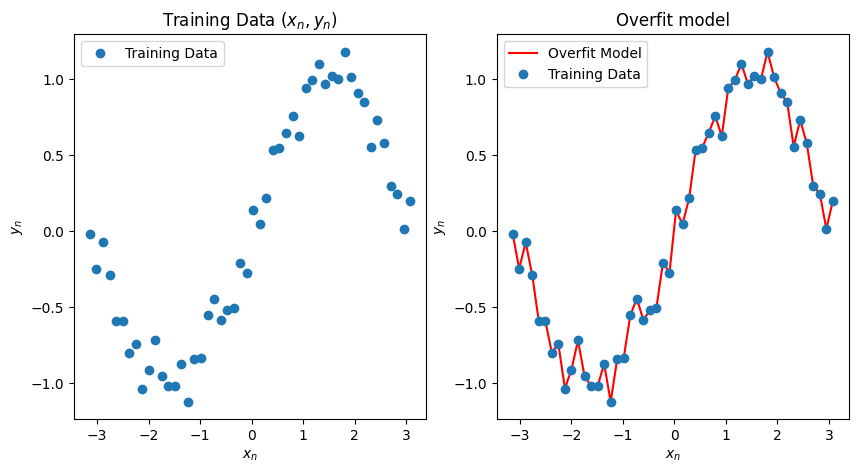
\includegraphics[width=0.9\textwidth]{figures/overfit.png}
\end{figure}
I.e. the overfit model learns to hit the training data points exactly.
In other words, the model is learning not only to approximate the underlying function, but also the noise in the data.

It is then natural to ask if this picture is really the case.

To make things more concrete, suppose that data is generated according to some process:

\begin{align*}
    y_n = f(x_n) + \varepsilon_n
\end{align*}

where $f$ is a deterministic function and $\varepsilon_n$ is a random error term with mean $0$.
Now, train a neural network $\hat{f}_\theta$ with parameters $\theta$ and overfit it to this data.
The question we ask is this:
If $X$ is a random variable that is distributed the same way as the distribution for the $x_n$'s, is it true that $\hat{f}_\theta(X) - f(X) \sim \varepsilon$?
I.e. is the residual of the overfit model on new data distributed the same way as the error term?

If the answer to this question is yes, we hypothesize that this may be an explanation for the phenomenon of deep double descent.
In this project, we attempt to answer the above question, and investigate deep double descent in the process.

\section{Increasing Network Width}
To start out, we generated 100 data points to train the models on.
The data was generated according to the following process:
\begin{align*}
    x_n &\sim \mathrm{Uniform}(-\pi, \pi) \\
    \varepsilon_n &\sim \mathrm{Normal}(0, 0.1) \\
    y_n &= \sin(x_n) + \varepsilon_n
\end{align*}
\begin{figure}[H]
    \centering
    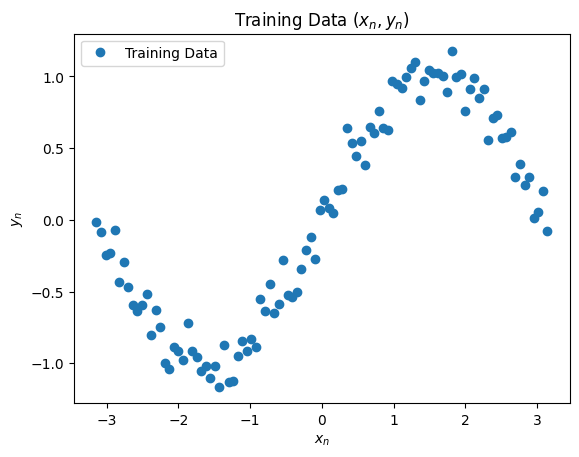
\includegraphics[width=0.9\textwidth]{figures/trainingdata.png}
\end{figure}
Then, we trained $\sim 200$ neural networks with a single hidden layer.
We varied the widths of the hidden layer of the networks from $100$ to $20,000$.
Then, using new data that was generated in the same way as the training data, we computed the residuals of the models on the new data.
The result was the following:
\begin{figure}[H]
    \centering
    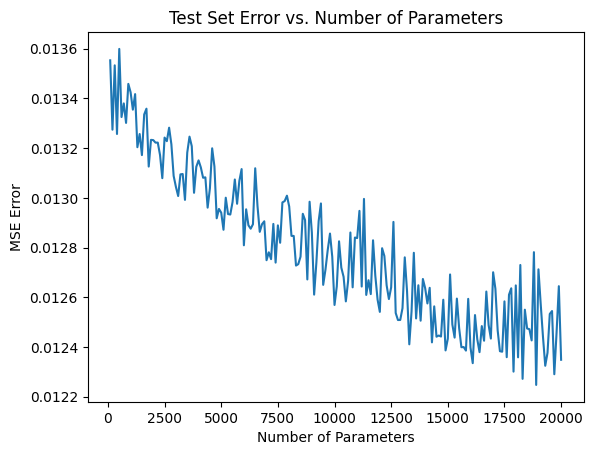
\includegraphics[width=0.9\textwidth]{figures/width.png}
\end{figure}
Note that there is a clear trend that shows that as the number of parameters increases, the magnitude of the residuals decreases.
This is not what we were expecting to see, as the standard picture of overfitting is that the model should learn to exactly hit the training data.
This would suggest that the residuals should increase with the number of parameters \emph{unless} double descent is happening.
However, we did not see double descent in this case either.

This led us into investigating under what circumstances double descent occurs.
This will be addressed later in the report.

To see whether $\hat{f}_\theta(X) - f(X) \sim \varepsilon$, we plotted the KL divergence between the distribution of $\hat{f}_\theta(X) - f(X)$ and the distribution of $\varepsilon$ as the number of parameters increased.
This gave the following results:
\begin{figure}[H]
    \centering
    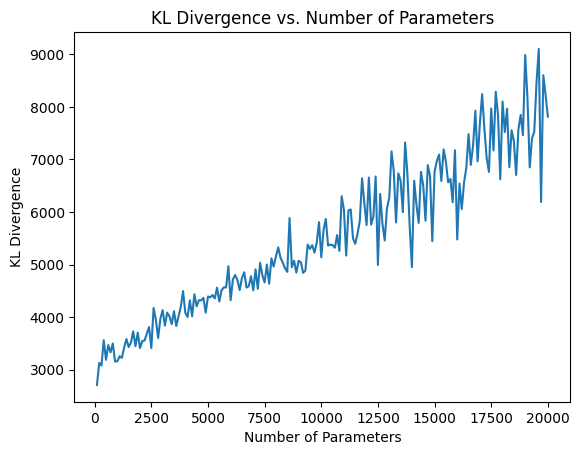
\includegraphics[width=0.9\textwidth]{figures/klwidth.png}
\end{figure}
As can be seen in the figure, the KL divergence actually \emph{increases} as the number of parameters increases.
This would suggest that the distribution of $\hat{f}_\theta(X) - f(X)$ is not converging to the distribution of $\varepsilon$, at least for a single hidden layer network.

Looking at the plot of $\hat{f}_\theta(X)$ for the $20,000$-wide model shows why this is the case.

\begin{figure}[H]
    \centering
    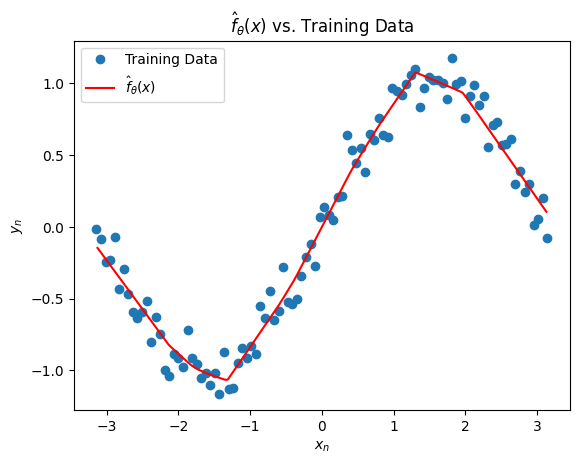
\includegraphics[width=0.9\textwidth]{figures/width20000.png}
\end{figure}

It appears that the model overfitting is not behaving as the standard picture would suggest.
Instead of learning to hit the training data exactly, it is learning to approximate the underlying function.
This is why the KL divergence is increasing as the number of parameters increases.
\end{document}